\subsection{Free-Space Scenario}
\label{subsec:exp2-free-space}

The free-space scenario serves as the baseline because it has no building blockage; distance is the sole large-scale factor.
UEs are distributed up to $1000$~m from the gNB, so the scenario combines strong near-field links with very weak cell-edge links.

\subsubsection{Application-related Metrics}
\label{subsubsec:exp2-free-space-flow}

Figure~\ref{fig:exp2-free-space-flow} shows per-application throughput, packet loss, delay, and jitter for both directions and all antenna configurations.
The stochastic ns-3 model outperforms Sionna~RT in average downlink throughput: at $8\times8$, ns-3 delivers $4.85$~Mbit/s ($21.6\%$ loss) versus $3.77$~Mbit/s ($26.6\%$ loss) for Sionna~RT, with the same ordering at $2\times2$.
The gap reflects the large cell radius: UEs at the cell edge experience greater path loss under ray tracing than the stochastic model predicts.
Array scaling yields only marginal throughput gain in both simulators because the bottleneck is cell-edge path loss, not beamforming resolution.

\begin{figure*}[t]
    \centering
    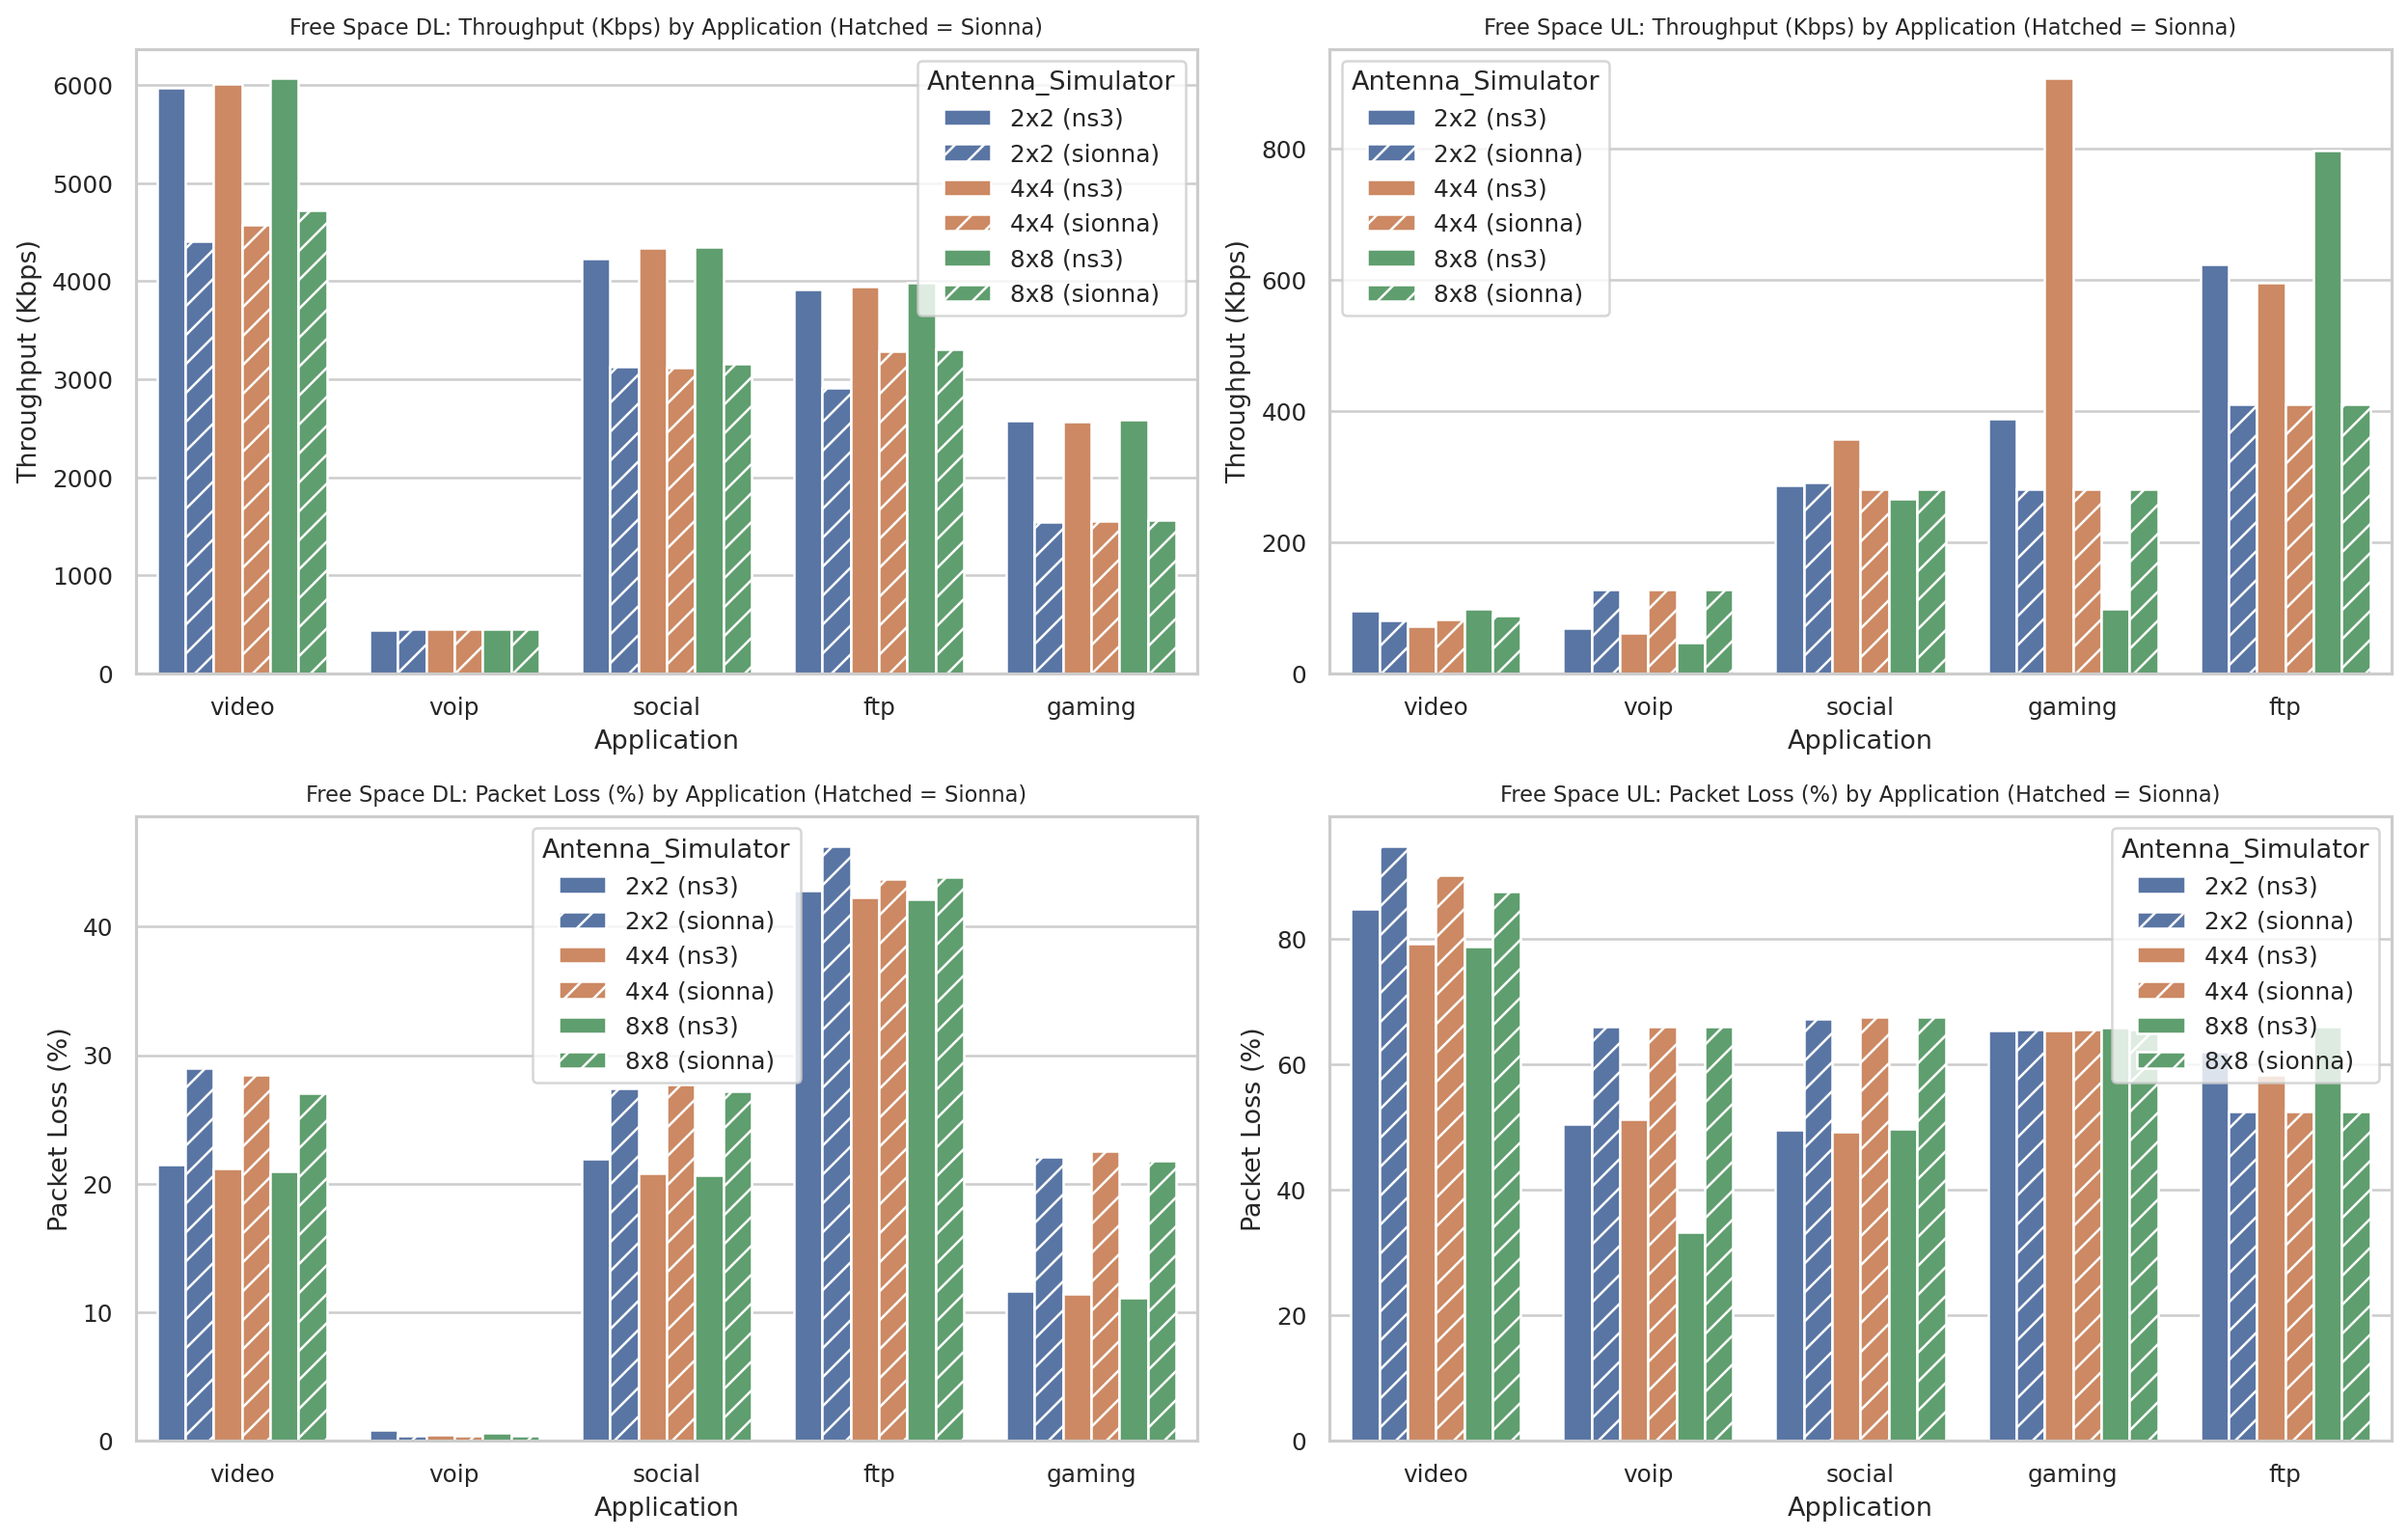
\includegraphics[width=\textwidth]{images/free_space_flow_metrics.png}
    \caption{Free-space application-level throughput and packet loss by application, direction, and gNB array size. Solid bars: ns-3; hatched bars: Sionna~RT.}
    \label{fig:exp2-free-space-flow}
\end{figure*}

\subsubsection{Propagation-related Metrics}
\label{subsubsec:exp2-free-space-propagation}

Average path loss is $94.2$~dB and estimated receive power is $-48.2$~dBm for both channel models (Fig.~\ref{fig:exp2-channel-quality}).
The ns-3 model reports a mean path delay of $3059$~ns while Sionna~RT reports $2237$~ns; both are consistent with radio path lengths of hundreds of metres.
CQI and MCS improve monotonically with array size in both simulators.
At $8\times8$, ns-3 reaches mean CQI~$15$ and MCS~$27$; Sionna~RT reaches CQI~$14.79$ and MCS~$26.59$.
The gap is small in free space because most links are near-line-of-sight; array gain raises channel quality but cannot overcome path loss for the most remote UEs.

\subsubsection{Energy Consumption-related Metrics}
\label{subsubsec:exp2-free-space-energy}

gNB power consumption increases with array size in both simulators (Fig.~\ref{fig:exp2-gnb-power}).
In ns-3, the gNB consumes $31.16$~W ($2\times2$), $64.58$~W ($4\times4$), and $199.39$~W ($8\times8$); Sionna~RT reports $30.08$~W, $59.08$~W, and $173.50$~W respectively.
UE power is similar across all configurations because the UE array is fixed at $2\times2$.
The throughput-per-watt trade-off is poor for larger arrays in this scenario: $8\times8$ consumes roughly six times the gNB power of $2\times2$ while delivering only marginal throughput gains.
Array gain cannot offset the scheduling pressure of serving many long-distance UEs under high traffic load.
